

The problem in matrix form is
\[
\min_x c^Tx
\]
subject to
\[
Ax= b,
\]
where
\[
 A \in \mathbb{R}^{2\times 4},\; b \in \mathbb{R}^2,\; c \in
 \mathbb{R}^4,\; x \in \mathbb{R}^4,
\]
\[
A =
\begin{pmatrix*}[r]
1&1&1&0\\
-1&2&0&1
\end{pmatrix*},
b =
\begin{pmatrix*}[r]
1\\
2
\end{pmatrix*},
c =
\begin{pmatrix*}[r]
1\\
0 \\
0 \\
0
\end{pmatrix*}.
\]
We have a problem with $n=4$ variables and $m=2$ equality constraints.
We consider the basic solution where $x_1$ and $x_2$ are in the basis:
$$
B =
\begin{pmatrix*}[r]
1&1\\
-1&2
\end{pmatrix*}
;
B^{-1} =
\begin{pmatrix*}[r]
\frac{2}{3}&-\frac{1}{3}\\
\frac{1}{3} & \frac{1}{3}
\end{pmatrix*}
;
x_B=B^{-1}b=
\begin{pmatrix*}[r]
0\\
1
\end{pmatrix*}
;
x
=
\begin{pmatrix}
0\\
1\\
0\\
0
\end{pmatrix}.
$$
The basic entries of the basic direction corresponding to the non basic variable $x_3$ is
calculated as
\[
-B^{-1} A_3 = -\begin{pmatrix*}[r]
\frac{2}{3}&-\frac{1}{3}\\
\frac{1}{3} & \frac{1}{3}
\end{pmatrix*} \cvect{1 \\ 0} = \cvect{-\frac{2}{3} \\ -\frac{1}{3}}.
\]
Therefore, the basic direction is
\[
d_3 = \cvect{-\frac{2}{3} \\ -\frac{1}{3} \\ 1 \\ 0}.
\]
 It is represented in the following
figure. 

\begin{center}
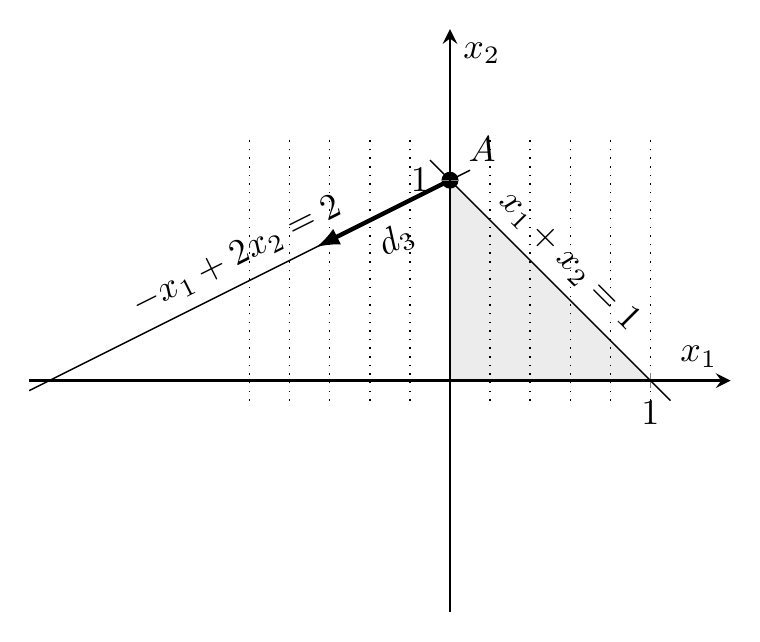
\begin{tikzpicture}[scale=1.3]
\begin{axis}[ xlabel={$x_1$}, ylabel={$x_2$}
    ,axis lines=middle
    ,axis equal
    ,axis on top=true
    ,xtick = {1}
    ,ytick = {1}
,samples=41, thick,
,domain=-0.5:8, xmin=-2.1, xmax=1.4,
    ymin=-0.5, ymax=1.1,
]
\fill[lightgray!30] (0,0) -- (0,1) -- (1,0) -- (0,0) -- cycle;
\addplot+ [mark=none,mark color=black, color=black, thin,domain=-0.1:1.1]{1-x}node[pos=0.5,sloped,above] {$x_1+x_2=1$};
\addplot+ [mark=none,mark color=black, color=black, thin,domain=-2.1:0.1]{1+0.5*x}node[pos=0.5,sloped,above] {$-x_1+2x_2=2$};
\draw (0,5) circle[radius=2.2pt];
\fill (0,5)  circle[radius=2.2pt];
\node [circle,fill=black,draw,scale=0.2,label=above right:$A$] at
(0,1) {A};
\draw[-latex,very thick] (0,1) -- (-2/3,2/3)
node[pos=0.5,below,sloped] {$d_3$};
\pgfplotsinvokeforeach{-1,-0.8,...,1} {\draw[dotted,thin] (#1,-0.1)
  -- (#1,1.2);}
\end{axis}
\end{tikzpicture}
\end{center}

The slope of the objective function is given by the directional
derivative. As
\[
c = \cvect{1 \\ 0 \\ 0 \\ 0}
\]
we have
\[
d_3^T c = -\frac{2}{3}.
\]
It is negative. It means that the objective function is decreasing
along that direction. 
The reduced cost is
\[
\bar{c}_3 = c_3 - c_B^T B^{-1} A_3 = 0 - (1 \; 0) \begin{pmatrix*}[r]
\frac{2}{3}&-\frac{1}{3}\\
\frac{1}{3} & \frac{1}{3}
\end{pmatrix*} \cvect{1 \\ 0} = -\frac{2}{3},
\]
and we confirm that it is indeed the slope of the function in the
basic direction. 

The basic entries of the basic direction corresponding to the non basic variable $x_4$ is
calculated as
\[
-B^{-1} A_4 = -\begin{pmatrix*}[r]
\frac{2}{3}&-\frac{1}{3}\\
\frac{1}{3} & \frac{1}{3}
\end{pmatrix*} \cvect{0 \\ 1} = \cvect{\frac{1}{3} \\ -\frac{1}{3}}.
\]
Therefore, the basic direction is
\[
d_4 = \cvect{\frac{1}{3} \\ -\frac{1}{3} \\ 0 \\ 1}.
\]
It is represented in the following figure. 

\begin{center}
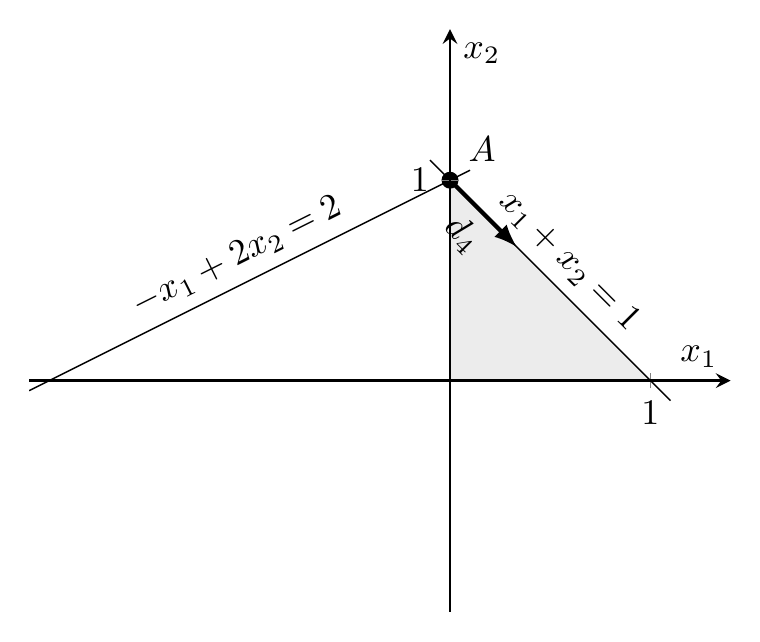
\begin{tikzpicture}[scale=1.3]
\begin{axis}[ xlabel={$x_1$}, ylabel={$x_2$}
    ,axis lines=middle
    ,axis equal
    ,axis on top=true
    ,xtick = {1}
    ,ytick = {1}
,samples=41, thick,
,domain=-0.5:8, xmin=-2.1, xmax=1.4,
    ymin=-0.5, ymax=1.1,
]
\fill[lightgray!30] (0,0) -- (0,1) -- (1,0) -- (0,0) -- cycle;
\addplot+ [mark=none,mark color=black, color=black, thin,domain=-0.1:1.1]{1-x}node[pos=0.5,sloped,above] {$x_1+x_2=1$};
\addplot+ [mark=none,mark color=black, color=black, thin,domain=-2.1:0.1]{1+0.5*x}node[pos=0.5,sloped,above] {$-x_1+2x_2=2$};
\draw (0,5) circle[radius=2.2pt];
\fill (0,5)  circle[radius=2.2pt];
\node [circle,fill=black,draw,scale=0.2,label=above right:$A$] at
(0,1) {A};
\draw[-latex,very thick] (0,1) -- (1/3,2/3)
node[pos=0.5,below,sloped] {$d_4$};
\end{axis}
\end{tikzpicture}
\end{center}

The slope of the objective function is given by the directional
derivative. As
\[
c = \cvect{1 \\ 0 \\ 0 \\ 0}
\]
we have
\[
d_4^T c = \frac{1}{3}.
\]
It is positive. It means that the objective function is increasing
along that direction. 
The reduced cost is
\[
\bar{c}_4 = c_4 - c_B^T B^{-1} A_4 = 0 - (1 \; 0) \begin{pmatrix*}[r]
\frac{2}{3}&-\frac{1}{3}\\
\frac{1}{3} & \frac{1}{3}
\end{pmatrix*} \cvect{0 \\ 1} = \frac{1}{3},
\]
and we confirm that it is indeed the slope of the function in the
basic direction. 

We have calculated the reduced costs for the two non basic
variables. We now need to calculate them for the basic variables.
\[
\bar{c}_1 = c_1 - c_B^T B^{-1} A_1 = 1 - (1 \; 0) \begin{pmatrix*}[r]
\frac{2}{3}&-\frac{1}{3}\\
\frac{1}{3} & \frac{1}{3}
\end{pmatrix*} \cvect{1 \\ -1} = 0,
\]
and
\[
\bar{c}_2 = c_2 - c_B^T B^{-1} A_2 = 0 - (1 \; 0) \begin{pmatrix*}[r]
\frac{2}{3}&-\frac{1}{3}\\
\frac{1}{3} & \frac{1}{3}
\end{pmatrix*} \cvect{1 \\ 2} = 0.
\]
This confirms the fact that the reduced costs of basic variables is
always zero.

